\documentclass[12pt]{article}
\usepackage[utf8]{inputenc}
\usepackage[english]{babel}
\usepackage[
	hidelinks,
	colorlinks,
	linkcolor=blue,
	citecolor=blue,
	urlcolor=blue,
]{hyperref}
\usepackage{booktabs}
\usepackage{amsmath}
\usepackage{xcolor}
\usepackage[ruled]{algorithm2e}
\usepackage{pgfplots}
\usepgfplotslibrary{groupplots}
\pgfplotsset{compat=newest}

\begin{document}

\title{
	Disperse Protocol\\
	\Large{Optimizing gas costs of ERC-20 token transfers}
}
\author{Artem K\\ \small{banteg@protonmail.com}}

\maketitle
\abstract{
This paper dissects the gas costs incurred when transferring tokens on EVM\footnote{Ethereum Virtual Machine}-based networks and discusses the possible optimization strategies.
It presents a concise smart contract for batch sending both native and ERC-20 tokens. 
It argues about the design decisions that would allow to fit 2--3x more transfers in a single block.
We also discuss how the token developers optimize for gas usage and provide benchmarks against Byzantium and Constantinople virtual machines.
}

\section{Background}
Ethereum is a decentralized ledger that allows arbitrary programs to run on its virtual machine.
These programs are called smart contracts.
In addition to balance and nonce, contract accounts have an associated EVM code and storage.
A contract can chain calls to other contracts allowing for complex interactions.\cite{ethereum}

The base unit of computation is called gas.
Program execution is instrumented with each opcode having its own gas cost.
The user provides a gas limit and a gas price, the maximum amount of computation allowed and the cost per unit of gas respectively.
Transaction fee is the product of the actual gas used and the gas price.

ERC-20 is a community-developed standard interface for fungible tokens\cite{eip20}.
Such contracts keep track of user balances in its storage and make the corresponding updates on each successful \textbf{transfer} function call.
The state-changing operations are are disincentivized with higher gas costs.

A lot of effort is currently directed at scaling Ethereum.
This paper proposes a ready-to-use batching protocol for both native (ETH) and ERC-20 tokens which allows to fit 2--3x more transfers in a single block.
It can aid heavy gas consumers like centralized exchanges to significantly cut their costs.

\section{Sending tokens}
\subsection{Single transfers}
The simplest token contract consists of a mapping containing user balances and a \textbf{transfer} function that updates it:
%
\begin{center}
	balances = $(address \rightarrow uint256)$
\end{center}
%
Sending a transaction with the attached data to the address that contains code is used to invoke a program.
Programs written in Solidity expect data to begin with a four-byte function signature with the rest being the function arguments.

The signature of a function is computed by taking the first four bytes of the keccak hash of the function name and argument types. In this case:
\begin{center}
	function = ``transfer(address,uint256)'' \\
	signature = bytes4(keccak256(function)) = a9059cbb
\end{center}

The arguments are tightly packed and padded to EVM word size of 32 bytes, so a 20-byte address is encoded with 12 leading zero bytes and a number is encoded as a 256-bit big-endian unsigned integer.

Each successful token transfer updates the balances for both the sender and the recipient and emits a \textbf{Transfer} event.
The event contains three indexed log topics (event signature, sender and recipient) and the raw data field with the amount sent.
The topics are added to the block's bloom filter which allows for efficient search and filtering.

%The event signature is computed like this:
%\begin{center}
%	event = ``Transfer(address,address,uint256)" \\
%	topic = keccak256(event) = 
%	\smaller{ddf252ad1be2c89b69c2b068fc378daa952ba7f163c4a11628f55a4df523b3ef}
%\end{center}

A user can give another account the right to spend up to a certain amount on her behalf. This concept is called allowance.
Allowances are stored as a map of addresses to spenders to their remaining allowance:
\begin{center}
	allowed = $(address \rightarrow (address \rightarrow uint256))$
\end{center}

A user invokes \textbf{approve} function with a spender address and a maximum allowance as the arguments.
Then the spender can transfer the tokens by calling \textbf{transferFrom} passing the user address, a recipient and a value.

This is a common pattern for interacting with smart contracts.
Instead of calling \textbf{transfer} function, which doesn't notify the recipient, the user calls a contract which chains the call to the token contract's \textbf{transferFrom} and makes the operation on behalf of the user.

\subsection{Estimating gas costs}

\begin{table}[h]
\caption{Ethereum gas schedule\cite{yellowpaper}}
\label{gas-costs}
\begin{center}
\begin{tabular}{l r l}
	Name & Value & Description \\ \midrule
	$G_{transaction}$ & 21000 \\
	$G_{sload}$ & 200 \\
	$G_{sstore}$ & 5000 & if value was non-zero \\
	$G_{sstore}$ & 20000 & if value was zero \\
	$G_{log}$ & 375 \\
	$G_{logtopic}$ & 375 \\
	$G_{logdata}$ & 8 & per byte \\
	$G_{txdatazero}$ & 4 & per zero byte \\
	$G_{txdatanonzero}$ & 68 & per non-zero byte \\
\end{tabular}
\end{center}
\end{table}
%
Let's break down the most expensive operations during \textbf{transfer}.
For gas costs see Table~\ref{gas-costs}.

\begin{enumerate}
	\item Invoke a transaction: $G_{transaction}$
	\item Cost of the attached data: $68 \cdot (G_{txdatanonzero} + G_{txdatazero})$
	\item Load the balances: $2 \cdot G_{sload}$
	\item Store the updated balances: $2 \cdot G_{sstore}$
	\item Emit the Transfer event: $G_{log} + 3 \cdot G_{logtopic} + 32 \cdot G_{logdata}$
\end{enumerate}

There is more logic involved, but the rest is cheap enough to ignore in this estimation.

We assume that the address contains no zero bytes which is the most common case.

Balances are stored in the lowest denomination as unsigned 256-bit integers.
Most tokens go for 18 decimal points taking after the native currency (1 ether = $10^{18}$ wei).
The median transfer value across the recent transfers on Ethereum mainnet is $10^{20}$ wei (100 tokens), we'll use that value in our tests.

With these assumptions the data passed along with the transaction has 31 non-zero and 37 zero bytes:
\begin{equation}
	G_{data} = 31 \cdot G_{txdatanonzero} + 32 \cdot G_{txdatazero} = 2256 \text{ gas}
\end{equation}

It's safe to assume that the sender's token balance is non-zero, so the only variable left is whether the recipient's balance was zero.
This leaves us with a ballpark estimation of 35,412--50,412 gas:
\begin{gather}
	G_{transaction}^{21000} + G_{data}^{2256} + G_{sload}^{400} + G_{sstore}^{10000} + G_{log}^{1756} = 35412 \text{ gas} \\
	G_{transaction}^{21000} + G_{data}^{2256} + G_{sload}^{400} + G_{sstore}^{25000} + G_{log}^{1756} = 50412 \text{ gas}
\end{gather}
%
This is not far from truth, the widely-used OpenZeppelin\cite{openzeppelin} ERC-20 implementation consumes 36,947--51,947 gas.
It is possible to fit 154--216 transfers in a block with the current block gas limit of  8,000,000.

The gas cost for \textbf{transferFrom} function is in range of 44,400--59,400, or up to 134--180 transfers per block. The biggest addition is 5000 gas for updating allowance.

\section{Batch transfers}
\subsection{Simple approach}

The gas costs can be reduced by invoking multiple transfers at once.
A simple approach is to create a contract that receives a token address, a list of recipients and a list of values and calls token's \textbf{transferFrom} while iterating over recipients and values pairwise. 
This allows to to pay $G_{transaction}$ just once which makes a significant difference when approaching the block gas limit.

Algorithm \ref{simple} is based on a simplified Multiplexer contract\cite{multiplexer}.
It removes the unnecessary assumptions about the recipients and values arrays as transaction reverts on out of bounds access anyway\cite{solidity-errors}.
It also uses uint256 instead of uint8 for iterator variable which saves some gas because no additional type conversion is required.

One such transaction could accommodate 206--337 transfers with an average gas cost of 23,694--38,739 per transfer. 
This is already a 1.34--1.56x improvement over direct transfers.

\begin{algorithm}[h]
\SetKwInOut{Input}{input}
\label{simple}
\caption{Disperse ERC-20 tokens using transferFrom}
\Input{token, recipients, values}
\BlankLine
\For{$i \in [0 \dots \text{recipients.length})$}{
	require(token.transferFrom(sender, recipients[i], values[i]))
}
\end{algorithm}

\subsection{Optimized approach}

A contract can use just one \textbf{transferFrom} to itself and then distribute the tokens from its own address using \textbf{transfer}. We can ensure atomicity by using a \textbf{require} statement that reverts the transaction if any of the transfers fails.

\begin{algorithm}[h]
	\label{optimized}
	\caption{Disperse ERC-20 tokens using transfer}
	\SetKwInOut{Input}{input}
	\BlankLine
	\Input{token, recipients, values}
	$total \leftarrow 0$ \\
	\For{$i \in [0 \dots recipients.length)$}{
		$total \leftarrow total + values[i]$
	}
	require(token.transferFrom(sender, this, total)) \\
	\For{$i \in [0 \dots recipients.length)$}{
		require(token.transfer(this, recipients[i], values[i]))
	}
\end{algorithm}

Despite the need to iterate over the list twice, Algorithm \ref{optimized} saves 5000 gas on each transfer because \textbf{allowance} is only touched once.
%The side effect of this approach is that the Transfer events will have the contract's address as a sender.

This approach allows to fit 242--449 transfers in a block and reduces the cost of one transfer to 17,813--32,928 gas.
This is a 1.58--2.07x improvement over regular transfers and 1.18-1.33x improvement over a simpler approach.

\subsection{Visual comparison}

Table \ref{table-byzantium} and Figure \ref{chart-byzantium} present a comparison of two methods with \textit{n} \textbf{transfer} transactions as a baseline.
The areas on the chart show the bounds of the worst (all recipients had zero token balances) and the best cases (everyone had a non-zero balance).

\begin{table}[h]
\caption{ERC-20 transfers with gas limit $\rightarrow$ 8,000,000}
\label{table-byzantium}
\begin{center}
\begin{tabular}{lrrr}
Method & Transfers & Gas/transfer & Transactions \\ \midrule
transfer & 154--216 & 36,947--51,947 & 154--216 \\
transferFrom & 134--180 & 44,400--59,400 & 134--180 \\
disperseTokenSimple & 206--337 & 23,694--38,739 & 1 \\
disperseToken & 242--449 & 17,813--32,928 & 1
\end{tabular}
\end{center}
\end{table}

\begin{figure}[h!]
\centering{
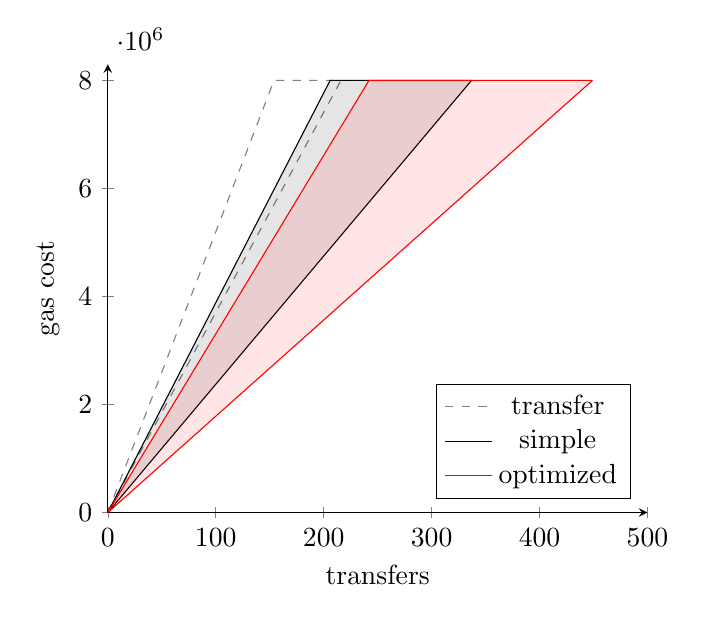
\begin{tikzpicture}
	\begin{axis}[
		xlabel=transfers,
		xmax=500,
		ymax=8300000,
		axis lines=left,
%		enlargelimits,
		legend pos=south east,
		ylabel=gas cost,
%		title=native token,
	]
    \addplot[forget plot, patch, dashed, faceted color=black!50, fill opacity=0]
    coordinates {
        (0, 0)
        (154, 8000000) % token transfer, zero balance 51947
		(216, 8000000) % token transfer, non-zero balance 36947
    };
    \addplot[forget plot, patch, black, faceted color=black, fill opacity=.1]
    coordinates {
        (0, 0)
		(206, 8000000) % disperse token, naive, zero balances, 206 recipients, 7980250 gas, 38739 gas/transfer
		(337, 8000000) % disperse token, naive, non-zero balances, 337 recipients, 7984991 gas, 23694 gas/transfer
    };
    \addplot[forget plot, patch, red, faceted color=red, fill opacity=.1]
    coordinates {
        (0, 0)
		(242, 8000000) % disperse token, optimized, zero balances, 242 recipients, 7968768 gas, 32928 gas/transfer
		(449, 8000000) % disperse token, optimized, non-zero balances, 449 recipients, 7998449 gas, 17813 gas/transfer
    };
    % for legend only
    \addplot[black!50, dashed] coordinates {(100, 0)};
    \addplot[black] coordinates {(100,0)};
    \addplot[red] coordinates {(100,0)};
    \legend{transfer, simple, optimized}
	\end{axis}
\end{tikzpicture}
}
\caption{Gas profile of Algorithms \ref{simple} and \ref{optimized}}
\label{chart-byzantium}
\end{figure}


\section{Further Optimization}

\subsection{Constantinople}

Constantinople is the name of Ethereum hard fork which is set to go live mid-January 2019.
It is already live on Ropsten testnet at the time of publication.
Among other improvements, the fork changes the gas metering rules for SSTORE,
discussed in EIP-1283\cite{eip1283}.

The new gas costs and refunds for writing to storage are based on the combination of three values: original, current and new.
The logic became much more complex, but the gist of it is that subsequent writes to the same storage slot during a single transaction became much cheaper.

This affects the proposed contract in a major way.
Consider the transitions of the contract token balance during the execution of an example transaction transferring three tokens to three recipients.

The number shows the balance value in storage. The upper number shows the gas cost of the SSTORE and the lower number shows the refund for clearing storage.
\begin{equation}
0 \xrightarrow{20000} 3 \xrightarrow{5000} 2 \xrightarrow{5000} 1 \xrightarrow[-15000]{5000} 0 = 20000 \text{ gas}	
\end{equation}

This is how it looks with EIP-1283 metering:
\begin{equation}
0 \xrightarrow{20000} 3 \xrightarrow{200} 2 \xrightarrow{200} 1 \xrightarrow[-19800]{200} 0 = 800 \text{ gas}	
\end{equation}

In generalized form with $n$ recipients:
\begin{gather}
G_{sset}^{20000} + n \cdot G_{sreset}^{5000} - R_{sclear}^{15000} = 5000 \cdot (n + 1) \\
G_{sset}^{20000} + n \cdot G_{snoop}^{200} - R_{sresetclear}^{19800} = 200 \cdot (n + 1)
\end{gather}

The new metering rules result in a 25x improvement of the total cost of updating the contract token balance.

See Table \ref{table-constantinople} and Figure \ref{eip1283-plot} for a comparison of how this change affects the performance of the proposed contract.


\begin{table}[h]
\caption{ERC-20 transfers with Constantinople VM}
\label{table-constantinople}
\begin{center}
\begin{tabular}{lrrr}
Method              & Transfers & Gas/transfer   & Transactions \\ \midrule
transfer            & 154--216  & 36,947--51,947 & 154--216     \\
transferFrom        & 134--180  & 44,400--59,400 & 134--180     \\
disperseTokenSimple & 274--568  & 14,082--29,145 & 1            \\
disperseToken       & 284--616  & 12,977--28,092 & 1           
\end{tabular}
\end{center}
\end{table}

\begin{figure}[h]
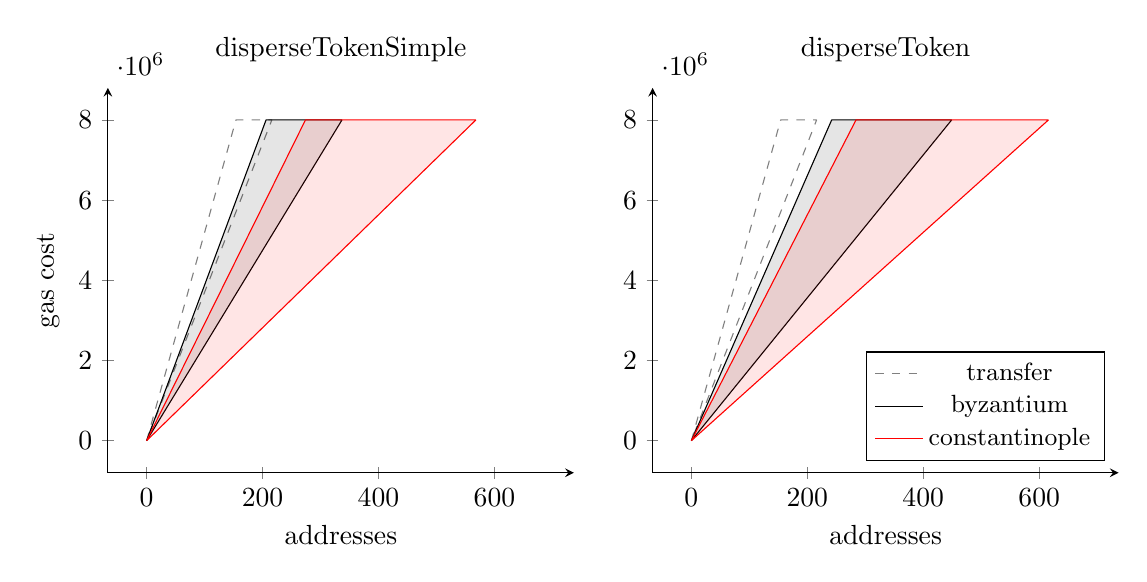
\begin{tikzpicture}
	\begin{groupplot}[
		width=7.5cm,
		xlabel=addresses,
		legend pos=south east,
		legend style={font=\small},
		xmax=670,
		axis lines=left,
		enlargelimits,
		group style={
			group size=2 by 1
		}
	]
	\nextgroupplot[ylabel=gas cost, title=disperseTokenSimple]
	\addplot[forget plot, patch, dashed, faceted color=black!50, fill opacity=0]
    coordinates {
        (0, 0)
        (154, 8000000)
		(216, 8000000)
    };
    \addplot[forget plot, patch, black, faceted color=black, fill opacity=.1]
    coordinates {
        (0, 0)
        (206, 8000000)
		(337, 8000000)
    };
    \addplot[forget plot, patch, red, faceted color=red, fill opacity=.1]
    coordinates {
        (0, 0)
		(274, 8000000)
		(568, 8000000)
    };
    \nextgroupplot[title=disperseToken]
    \addplot[forget plot, patch, dashed, faceted color=black!50, fill opacity=0]
    coordinates {
        (0, 0)
        (154, 8000000)
		(216, 8000000)
    };
    \addplot[forget plot, patch, black, faceted color=black, fill opacity=.1]
    coordinates {
        (0, 0)
        (242, 8000000)
		(449, 8000000)
    };
    \addplot[forget plot, patch, red, faceted color=red, fill opacity=.1]
    coordinates {
        (0, 0)
		(284, 8000000)
		(616, 8000000)
    };
    % for legend only
    \addplot[black!50, dashed] coordinates {(0, 0)};
    \addplot[black] coordinates {(0, 0)};
    \addplot[red] coordinates {(0, 0)};
    \legend{transfer, byzantium, constantinople}
	\end{groupplot}
\end{tikzpicture}
\caption{EIP-1283 effect on algorithms \ref{simple} and \ref{optimized}}
\label{eip1283-plot}
\end{figure}

The overall effect is improvement from 242--449 transfers to 284--616 for optimized approach, which is 1.17--1.37x better result and 1.84--2.85x improvement over non-batched transfers.


\subsection{Unlimited Allowance}
Allowance is oftentimes used as a binary switch.
A common pattern is to \textbf{approve} $\text{uint256}_{max}$ to indicate unlimited allowance:

\begin{center}	
\begin{tabular}{r l}
Allowance & Interpretation \\ \midrule
0 & Disabled  \\
$2^{256}-1$ & Enabled
\end{tabular}
\end{center}

There are at least two live ERC-20 tokens that optimize for gas usage using this pattern.
0x protocol's own ZRX token interprets $2^{256}-1$ as a magic value meaning ``unlimited allowance" and skips updating the allowance altogether in this case\cite{zrx-unlimited}.
This saves 5000 gas by skipping one SSTORE and makes the cost of \textbf{transfer} and \textbf{transferFrom} equal.

Another example is Wrapped Ether (WETH), which primary function is to trustlessly swap the native token to its ERC-20 form or back.



\section{Native Token}

Any value sent along with the transaction immediately becomes available as contract's own balance.
That's why it's important to keep track of how much was already sent to refund the excess value.

One way to approach this would be to calculate the total, similar to Algorithm~\ref{optimized}, but a more efficient method is to always ensure that the final contract balance remains zero after transaction.

\begin{algorithm}[h]
	\label{native}
	\caption{Disperse native token}
	\SetKwInOut{Input}{input}
	\BlankLine
	\Input{recipients, values}
	\For{$i \in [0 \dots recipients.length)$}{
		recipients[i].transfer(values[i])
	}
	$balance \leftarrow address(this).balance$ \\
	\If{$balance > 0$}{
	    msg.sender.transfer(balance)
	}
\end{algorithm}

Contract transfers use CALL\cite{subtleties} opcode which costs 7,400--32,400 gas, whereas a regular transaction costs a flat fee of 21,000 gas.
%
\begin{align}
G_{call}^{700} + G_{callvalue}^{9000} - G_{callstipend}^{2300} &= 7400 \\
G_{call}^{700} + G_{callvalue}^{9000} - G_{callstipend}^{2300} + G_{newaccount}^{25000} &= 32400
\end{align}

The $G_{newaccount}$ penalty makes it impractical to create new accounts using this algorithm, limiting the number of transfers in a block to 230, as opposed to 380 regular transfers.
This is 40\% worse result in terms of gas usage, but it is still one transaction instead of $n$.

Transferring to existing accounts from a contract allows to fit 830 transfers in a block, which is a massive 2.18x improvement over regular transfers.
Note that existing account may have zero balance.
The resulting cost per transfer is 9,629--34,701 gas.

Constantinople hard fork has no effect on sending native tokens.

\begin{table}[h]
\caption{Ethereum gas schedule}
\label{gas-costs-2}
\begin{center}
\begin{tabular}{l r l}
	Name & Value & Description \\ \midrule
	$G_{call}$ & 700 \\
	$G_{callvalue}$ & 9000 & if $value > 0$ \\
	$G_{callstipend}$ & 2300 & subtracted from $G_{callvalue}$ \\
	$G_{newaccount}$ & 25000 & if creates new account

\end{tabular}
\end{center}
\end{table}

\begin{table}[h]
\caption{Native token transfers with gas limit $\rightarrow$ 8,000,000}
\label{table-native}
\begin{center}
\begin{tabular}{@{}llll@{}}
Method        & Transfers & Gas/transfer  & Transactions \\ \midrule
call          & 380       & 21000         & 380          \\
disperseEther & 230--830  & 9,629--34,701 & 1           
\end{tabular}
\end{center}
\end{table}

\begin{figure}[h!]
\centering{
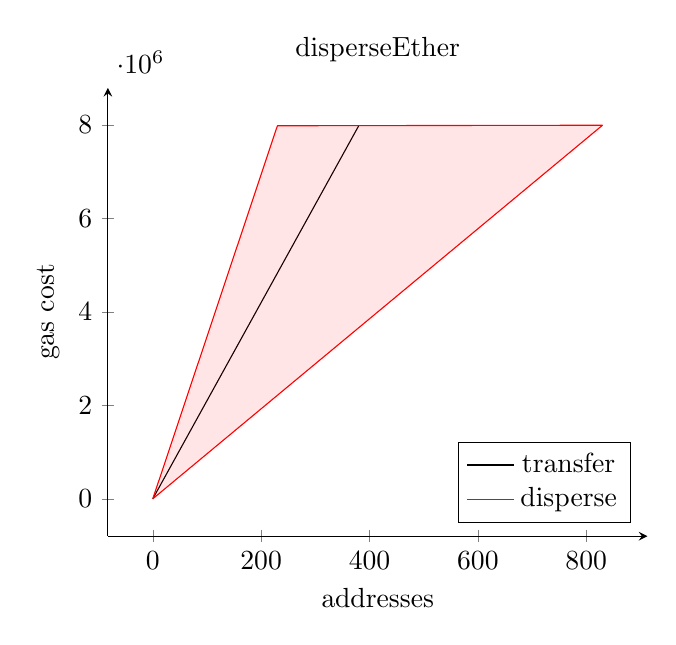
\begin{tikzpicture}
	\begin{axis}[
		xlabel=addresses,
		xmax=830,
		axis lines=left,
		enlargelimits,
		legend pos=south east,
		ylabel=gas cost,
		title=disperseEther,
	]
    \addplot[black, faceted color=black, fill opacity=.1]
    coordinates {
        (0, 0)
		(380, 7980000) % 21k
    };
    \addplot[forget plot, patch, red, faceted color=red, fill opacity=.1]
    coordinates {
        (0, 0)
		(230, 7981378) %disperse ether, zero balances, 230 recipients, 7981378 gas, 34701 gas/transfer
		(830, 7992706) %disperse ether, non-zero balances, 830 recipients, 7992706 gas, 9629 gas/transfer
    };
    % for legend only
    \addplot[red] coordinates {(100,0)};
    \legend{transfer, disperse}
	\end{axis}
\end{tikzpicture}
}
\caption{Gas profile of native token transfers}
\end{figure}


\section{Methodology}

Gas usage was instrumented using Py-EVM\cite{pyevm}.
The benchmark setup is built from low-level primitives which include only the virtual machine and an in-memory state database.
The setup allows testing against different forks by switching the virtual machine.
The mining and blockchain components are not used.

This allows to have full control over the underlying state and to read and write directly to the contract storage without the need to apply hundreds of transactions to prepare for each test case.

Storage is accessed by index, in the same order as defined in the Solidity source.
Mappings are accessed by keccak of their key and index, both of which are encoded as bytes32.
For example, \textbf{balances} mapping is accesses like this\cite{read-storage}:
\begin{center}
	keccak256(bytes32(address) + bytes32(0))	
\end{center}

Allowances are stored in the \textbf{allowed} mapping which can be accessed by repeating that twice:
\begin{center}
index = keccak256(bytes32(address) + bytes32(1)) \\
keccak256(bytes32(spender) + index)	
\end{center}

All tests use binary search to find the maximum number of transfers that can be fitted in a single block.
The complete test suite \href{https://github.com/banteg/disperse-reseach}{can be found on Github}.
There are also \href{https://github.com/banteg/disperse-reseach/tree/comparison}{additional tests} against other similar contracts.

\section{Conclusion}

We presented simple and optimal algorithms for batch sending both ERC-20 and native tokens and benchmarked them.

Batching results in 1.58--2.07x (1.84--2.87x after Constantinople) improvement in gas usage for tokens and 0.61--2.18x for ether transfers, see Tables \ref{table-byzantium}, \ref{table-constantinople}, \ref{table-native}.

A smart contract implementing Algorithms \ref{simple}, \ref{optimized}, \ref{native} is deployed on Ethereum mainnet and all its testnets as well as multiple other EVM-compatible networks at address:

\begin{center}
\href{https://etherscan.io/address/0xD152f549545093347A162Dce210e7293f1452150}{0xD152f549545093347A162Dce210e7293f1452150}	
\end{center}

There is also a client-only frontend interface which interacts with Metamask. It is hosted at \href{https://disperse.app/}{disperse.app}.


\begin{thebibliography}{1}

\bibitem{ethereum} \href{https://www.ethereum.org}{Ethereum Project, 2015}
 
 \bibitem{eip20} \href{https://eips.ethereum.org/EIPS/eip-20}{Fabian Vogelsteller, Vitalik Buterin. {\em EIP 20: ERC-20 Token Standard}, 2015}

 \bibitem{yellowpaper} \href{http://gavwood.com/paper.pdf}{Gavin Wood. {\em Ethereum: A Secure Decentralised Generalised Transaction Ledger}, Byzantium revision, 2017}

 \bibitem{openzeppelin} \href{https://github.com/OpenZeppelin/openzeppelin-solidity/blob/v2.0.0/contracts/token/ERC20/ERC20.sol#L151-L164}{OpenZeppelin-Solidity {\em Standard ERC20 token}, 2018}
   	
 \bibitem{multiplexer} \href{https://github.com/DigixGlobal/multiplexer}{DigixGlobal. {\em Multiplexer}, 2017}

 \bibitem{solidity-errors} \href{https://solidity.readthedocs.io/en/latest/control-structures.html#error-handling-assert-require-revert-and-exceptions}{Solidity Documentation. {\em Error handling in Solidity}, 2018}
 	
% \bibitem{cremer} \href{https://medium.com/p/d67bf08521ca}{Lukas Cremer. {\em Missing return value bug--At least 130 tokens affected}, 2018}
 	
 \bibitem{eip1283} \href{https://eips.ethereum.org/EIPS/eip-1283}{Wei Tang. {\em EIP 1283: Net gas metering for SSTORE without dirty maps}, 2018}

 \bibitem{zrx-unlimited} \href{https://github.com/0xProject/0x-monorepo/blob/48ff13e3e22bf9f71bc1a367f86aaa0ae89989ae/packages/contracts/contracts/tokens/ZRXToken/UnlimitedAllowanceToken_v1.sol#L43-L45}{0x Project. {\em Unlimited Allowance Token v1}, 2017}
 
\bibitem{subtleties} \href{https://github.com/ethereum/wiki/wiki/Subtleties}{Vitalik Buterin. {\em Ethereum Subtleties}, 2015}
 
\bibitem{pyevm} \href{https://github.com/ethereum/py-evm}{Py-EVM. {\em A Python implementation of the Ethereum Virtual Machine}, 2018}

\bibitem{read-storage} \href{https://medium.com/aigang-network/how-to-read-ethereum-contract-storage-44252c8af925}{Darius. {\em How to read Ethereum contract storage}, 2017}

\end{thebibliography}

\end{document}
